\documentclass[11pt,fleqn,twoside]{article}
\usepackage{makeidx}
\makeindex
\usepackage{palatino} %or {times} etc
\usepackage{plain} %bibliography style
\usepackage{amsmath} %math fonts - just in case
\usepackage{amsfonts} %math fonts
\usepackage{amssymb} %math fonts
\usepackage{lastpage} %for footer page numbers
\usepackage{fancyhdr} %header and footer package
\usepackage{mmpv2}
\usepackage{url}
\usepackage{graphicx}
% the following packages are used for citations - You only need to include one.
%
% Use the cite package if you are using the numeric style (e.g. IEEEannot).
% Use the natbib package if you are using the author-date style (e.g. authordate2annot).
% Only use one of these and comment out the other one.
\usepackage{cite}
%\usepackage{natbib}

\begin{document}

\name{Daniel Atkinson}
\userid{daa9}
\projecttitle{Arduino based obstacle avoidance robot}
\projecttitlememoir{Obstacle avoidance robot} %same as the project title or abridged version for page header
\reporttitle{Progress Report}
\version{0.1}
\docstatus{Draft}
\modulecode{CS39440}
\supervisor{Dave Barnes} % e.g. Neil Taylor
\supervisorid{dpb}
%\wordcount{}

%optional - comment out next line to use current date for the document
%\documentdate{26th October 2011}
\mmp

\setcounter{tocdepth}{3} %set required number of level in table of contents
\tableofcontents

\newpage

%==============================================================================
\section{Project Summary}
%==============================================================================
\subsection{Aim}
The aim of the project is to build and program an autonomous robot that can move around freely within an environment and avoid coliding with obstacles it may find.
\subsection{Background}
I tend to experiment with electronic components on a regular basis.  Due to this I try and make small systems and get them working, originaly nothing more than a simple timer or an audio amplifier.  Naturaly the progression from this would be to move onto microcontrollers.
\\I like to see things move, it keeps my interest.  The satisfaction I get when having started with nothing and going through to get something built and moving is what makes me think up new ideas, how can this be modified?, how can this be made better?.  A robotic project the perfect thing for me to do.
\\

%==============================================================================
\section{Current Progress}
%==============================================================================
\subsection{Related Works}
There are already lots of examples of work in this area.  Cameras can be used to find a path between objects using different image proccessing techniques.  These require a fairly high level of processing due to the amount of data in each image.  This can also sometimes lead to mistaking visible patterns in the environment as obstacles or empty space when there is none, such as a mirror or a patterned carpet. %Insert citation of roborealm example
\subsection{Technologies}

\subsubsection{Sensors}
\begin{itemize}
\item LDR (light dependant resistor)
\\Small resistor that changes its resistance depending on how much light it is exposed to.
\\This could be used to detect if the robot is very close to bumping into an object and avoid it as the object would shadow some of the light from getting to the resistor, like a bump skirt.
\item Camera
\\A camera could be used to detect objects in front of it using various image processing techniques.  This method is good because it can potentialy map a relatively large area in a single image.  On the other hand it requires more processing to do which can be slow and result in having colided into an object or being stuck in a tight space before it has finished processing. A camera and the proccessing linked to using it for obstacle avoidance also increases power consumption, decreasing total runtime.
\item Infra Red
\\Used to detect distance from an object.  An emiter and a reciever linked to work like the light dependant resistor but using infra red instead of visible light.  Depending on intensity it can be used to detect distance.  These could be aranged all around the robot like a halo to detect objects from all sides.
\item Sonar
\\Again emiter, reciever style approach.  Emit an ultrasonic wave to bounce off of whatever is in  front of the emitter and then time how long it takes to be picked up by the reciever to determine how far away the object is.  This method comes with its drawbacks.  Due to how sound waves behave when they interact with the environment by bouncing off of it.  If the surface is angled or curved the sound can bounce away from the reciever, either not returning to it at all and giving a false reading of there beign nothing in front of it, or be bouncing off of multiple objects back to the reciever giving a false longer reading than there actually is.
\end{itemize}
\subsubsection{Actuators}

\subsubsection{Materials}
I considered several materials for the robot chassis to be built of.
\begin{itemize}
\item Wood
\\This would be the easiest material to make the chassis from as it is cheap, easy to cut into the intended shape and easy to screw components to.  Also it being non-condictive would help when mounting circuit boards to it.
\item Plastic
\\The lighter option.  Good due to its low weight but not as strong as wood and could bend or snap under load of many of the heavier components such as motors or a power source.  Also can be more expensive than wood to aquire and cut into the desired shape.  It is also non-conductive, again useful to mount conponents to.
\item Steel
\\A stonger material that can take much heavier loads but is itself rather heavy compared to wood and plastic.  This extra weight will put more stress on the motors used to drive to robot and may even need the motors to be more powerfull.  It is conductive which means more materials will be needed to make a non-conductive mounting platform for electronic components.
\item Aluminium
\\A much lighter metal than the Steel, but still heavier than wood or plastic of the same thickness.  It can take heavier loads than the plastic. It is conductive, making it useless to mount components onto without a mounting platform of some kind.
\end{itemize}
Aluminium seems to be the best all round.  It is stong but not as heavy as steel.  It can act as a heat sink for the motos if they are mounted diectly.  Also it is not too expensive to buy in small amounts.
\\In addition to the aluminium base I have decided to use plastic for mounting components to the base.  To make this easier I have built at 3D printer for fabicating custom components to specification.

\subsubsection{Power Source}
As this robot is intended to move around freely the powersource cannot be supplied by an ordinaly power outlet, it has to be self contained.  This means it will have to be a battery.
\\The battery will have to be several cells or a single high output cell due to the size of motors I will be using.
\\I will need as many Amp hours as possible for longer runtimes.  This could be achieved with several cels linked together in series (end to end) to increase voltage and link more together in parrallel (side by side) to increase amp hours (runtime).
\\The lighter of the batteries would be to use lithium polymer (LiPo), these come in up to 11.2 volt packages which is not quite high enough to run the motors I have chosen.
\\A lead acid battery is the other choice with high enough output.  A single battery can output ~12 volts and can be supplied with high amp hour ratings compared to the lithium ion alternatives.
\\The chosen battery is rated at 12 volts and 4 amp hours.  It weighs more than the LiPo but is a more convenient package as it takes up less space on the robot.
\subsubsection{3D Printer}
As mentioned previously I have built a 3D printer.  This was not built exclusively to aid in this project but it was a factor in the puchase decision.
\\The printer was not designed by me, it was bought as a kit.  The construction of the device aided as a good learning proccess and deepened my understanding of how 3d printing works.
\\The build area of the printer is 200x200x260mm (length x width x depth) so it can produce fairly large components.
\begin{figure}[h]
\centering
        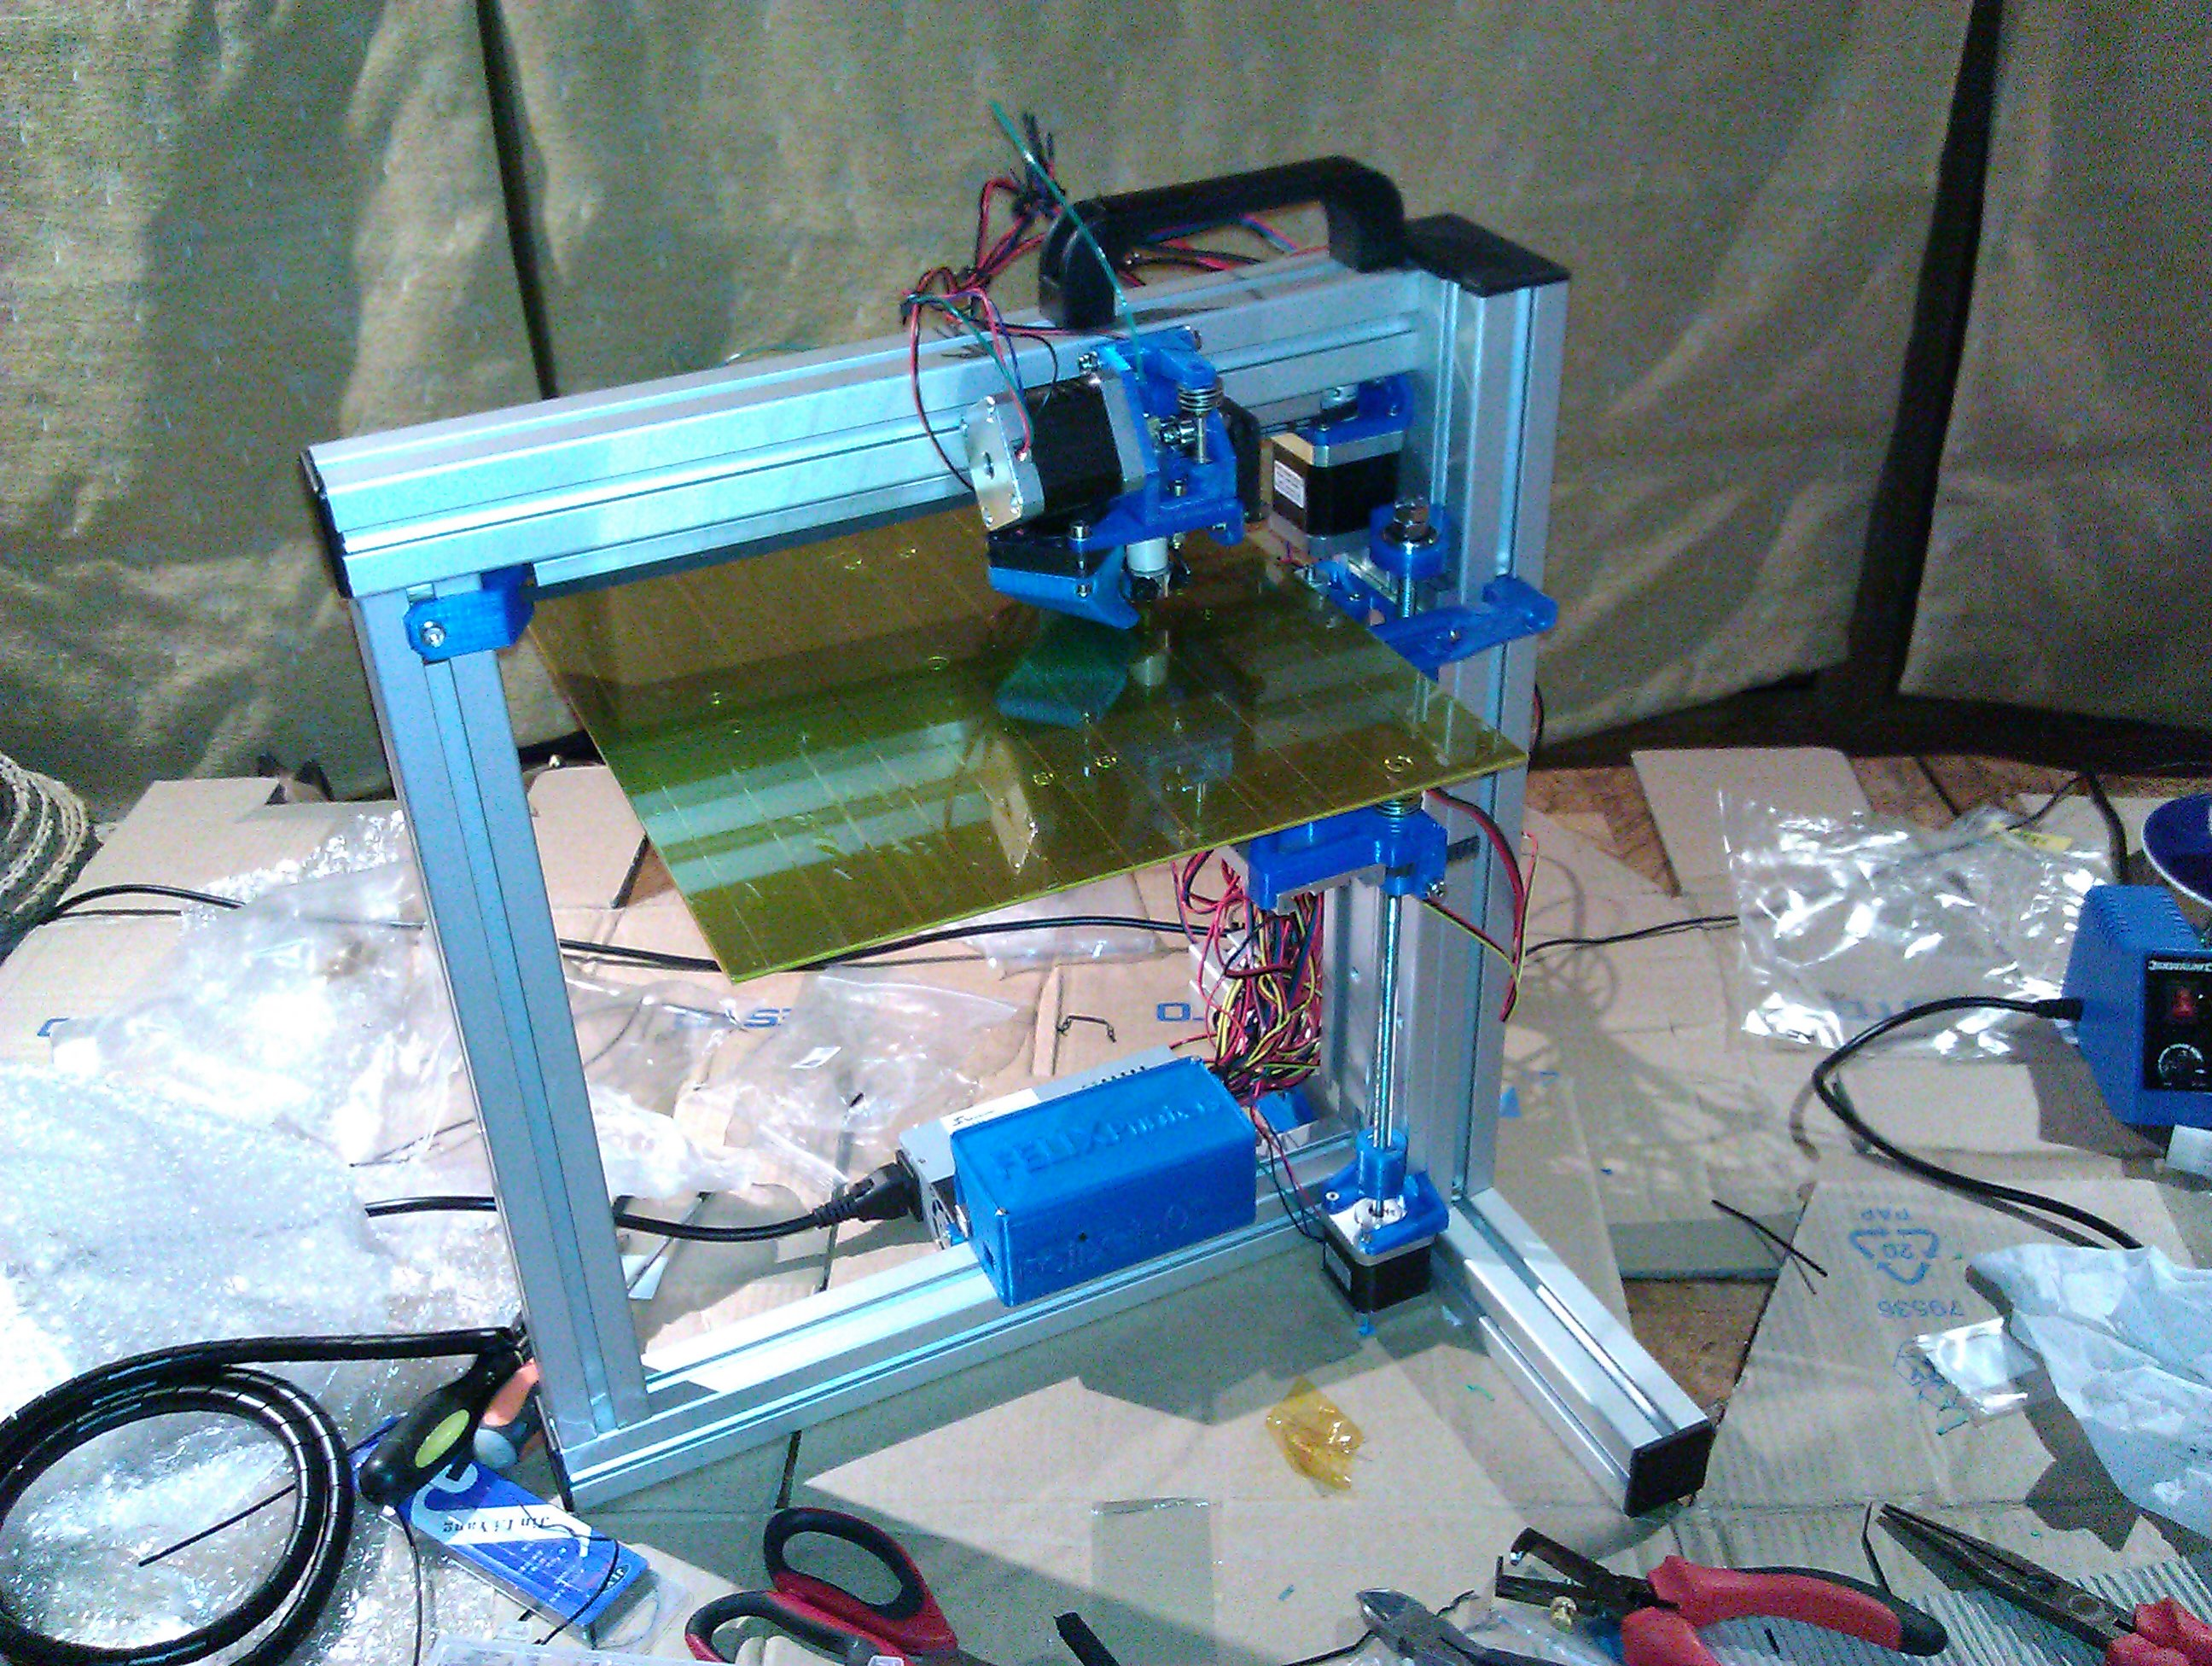
\includegraphics[width=5.0in] {figures/printer.jpg}
        \caption{3D Printer}
        \label{3D Printer}
\end{figure}



\subsection{Initial Learning}
After choosing to use the arduino due to it having such a vast amount of support and examples I bought one and began to learn how to use it, using the arduino website itself as a guide (arduino.cc).  On here there are many tutorials with circuit diagrams and example code on how to get the basics working, which I found very helpful.
\\The first things to learn were how to interact with the development board from my computer, then move onto getting it to output something.  Making lights blink was easy, and communicating over a serial connection was also relatively easy.  It got a bit harder when trying to recieve useful input from a sensor.
\\The first input I recieved was from an Infra Red sensor, using this to determine how far an object was from the sensor itself.
\\Something I discovered very quickly was that even if the sensor was not moved and the object it is pointing at is not mvoed the valus recieved from the sensor vary.  This 'noise' could cause a problem.  The obvious solution was to take a range of samples and average them to get a less eratic reading.
\\To further add to that I may add a threshold and if the value from each reading it too different from the current average of a range of the most recent readings, then discard that value as to not push the average.

Next I moved onto motors.  I had a 9 volt DC motor in the kit that came with my Arduino starter pack.  Getting the motor to turn was very easy, just apply current to one side and have the other linked to ground.  Simple.
\\Getting the motor to turn both forwards and backwards seemed liek it would be harder.  But due to this motor runnign well off of 5 volts this was not an issue as an Arduino can output around 5 volts on its output pins and also link these pins to ground as well.  As such I can just switch which pin is ground and which is supplying voltage to change the direction of the motor.  Of course this will not be so easy for larger motors as the Arduino will not be able to supply enough voltage in this manner.  I will require a motor driver.

\subsection{Prototype}
To build the prototype I bought a small plastic chassis kit which inclided the chassis, two wheels, a caster for the rear 'wheel', two motors and two sets of gears for the motors.  All I needed to add was the microcontroler itself, a motor driver and a power source to get this running.
%add picture of tria MK-I
\begin{figure}[h]
\centering
        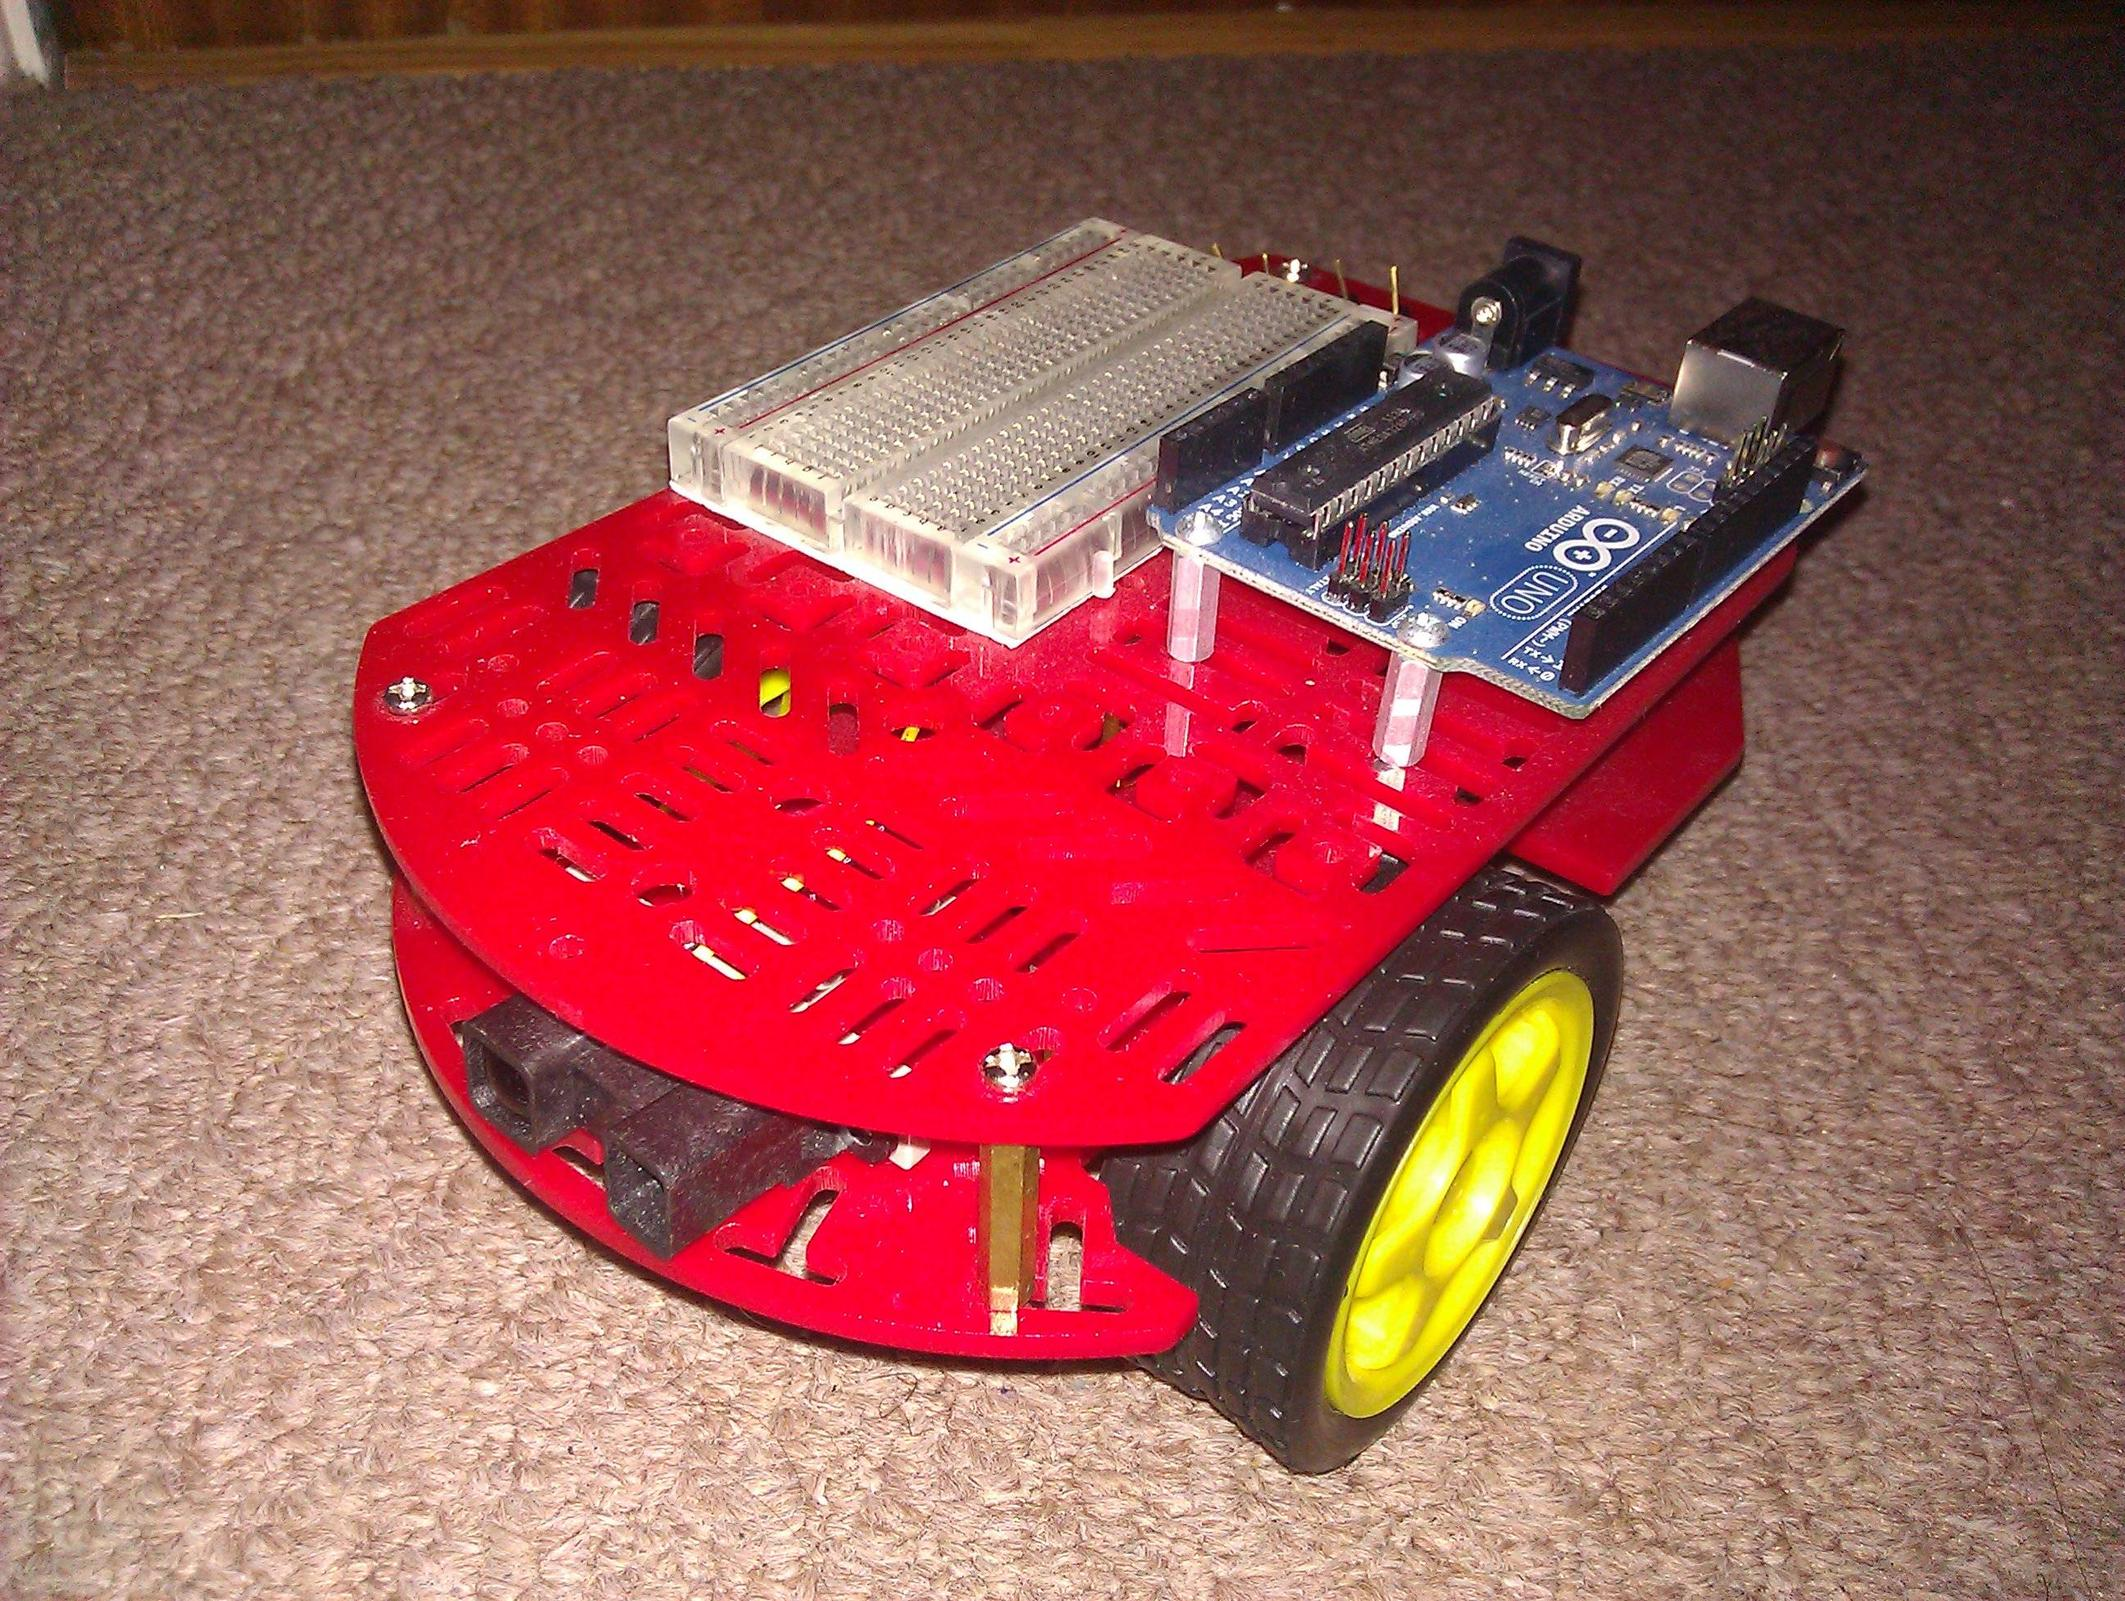
\includegraphics[width=5.0in] {figures/tria-mkI.jpg}
        \caption{Plastic prototype}
        \label{Plastic prototype}
\end{figure}

\subsection{Current Build}
So far a basic chassis has been built out of aluminium.  This consisted of cutting a sheet of aluminium to the desired shape, cutting two more pieces, bending them at a 90 degree angle and cutting a hole in them to mount the robots motors too.  These two pieces were then bolted onto the underside of the larger piece.  A further piece was bolted onto the base plate extruding out of the back to support a rear wheel.
\begin{figure}[h]
\centering
        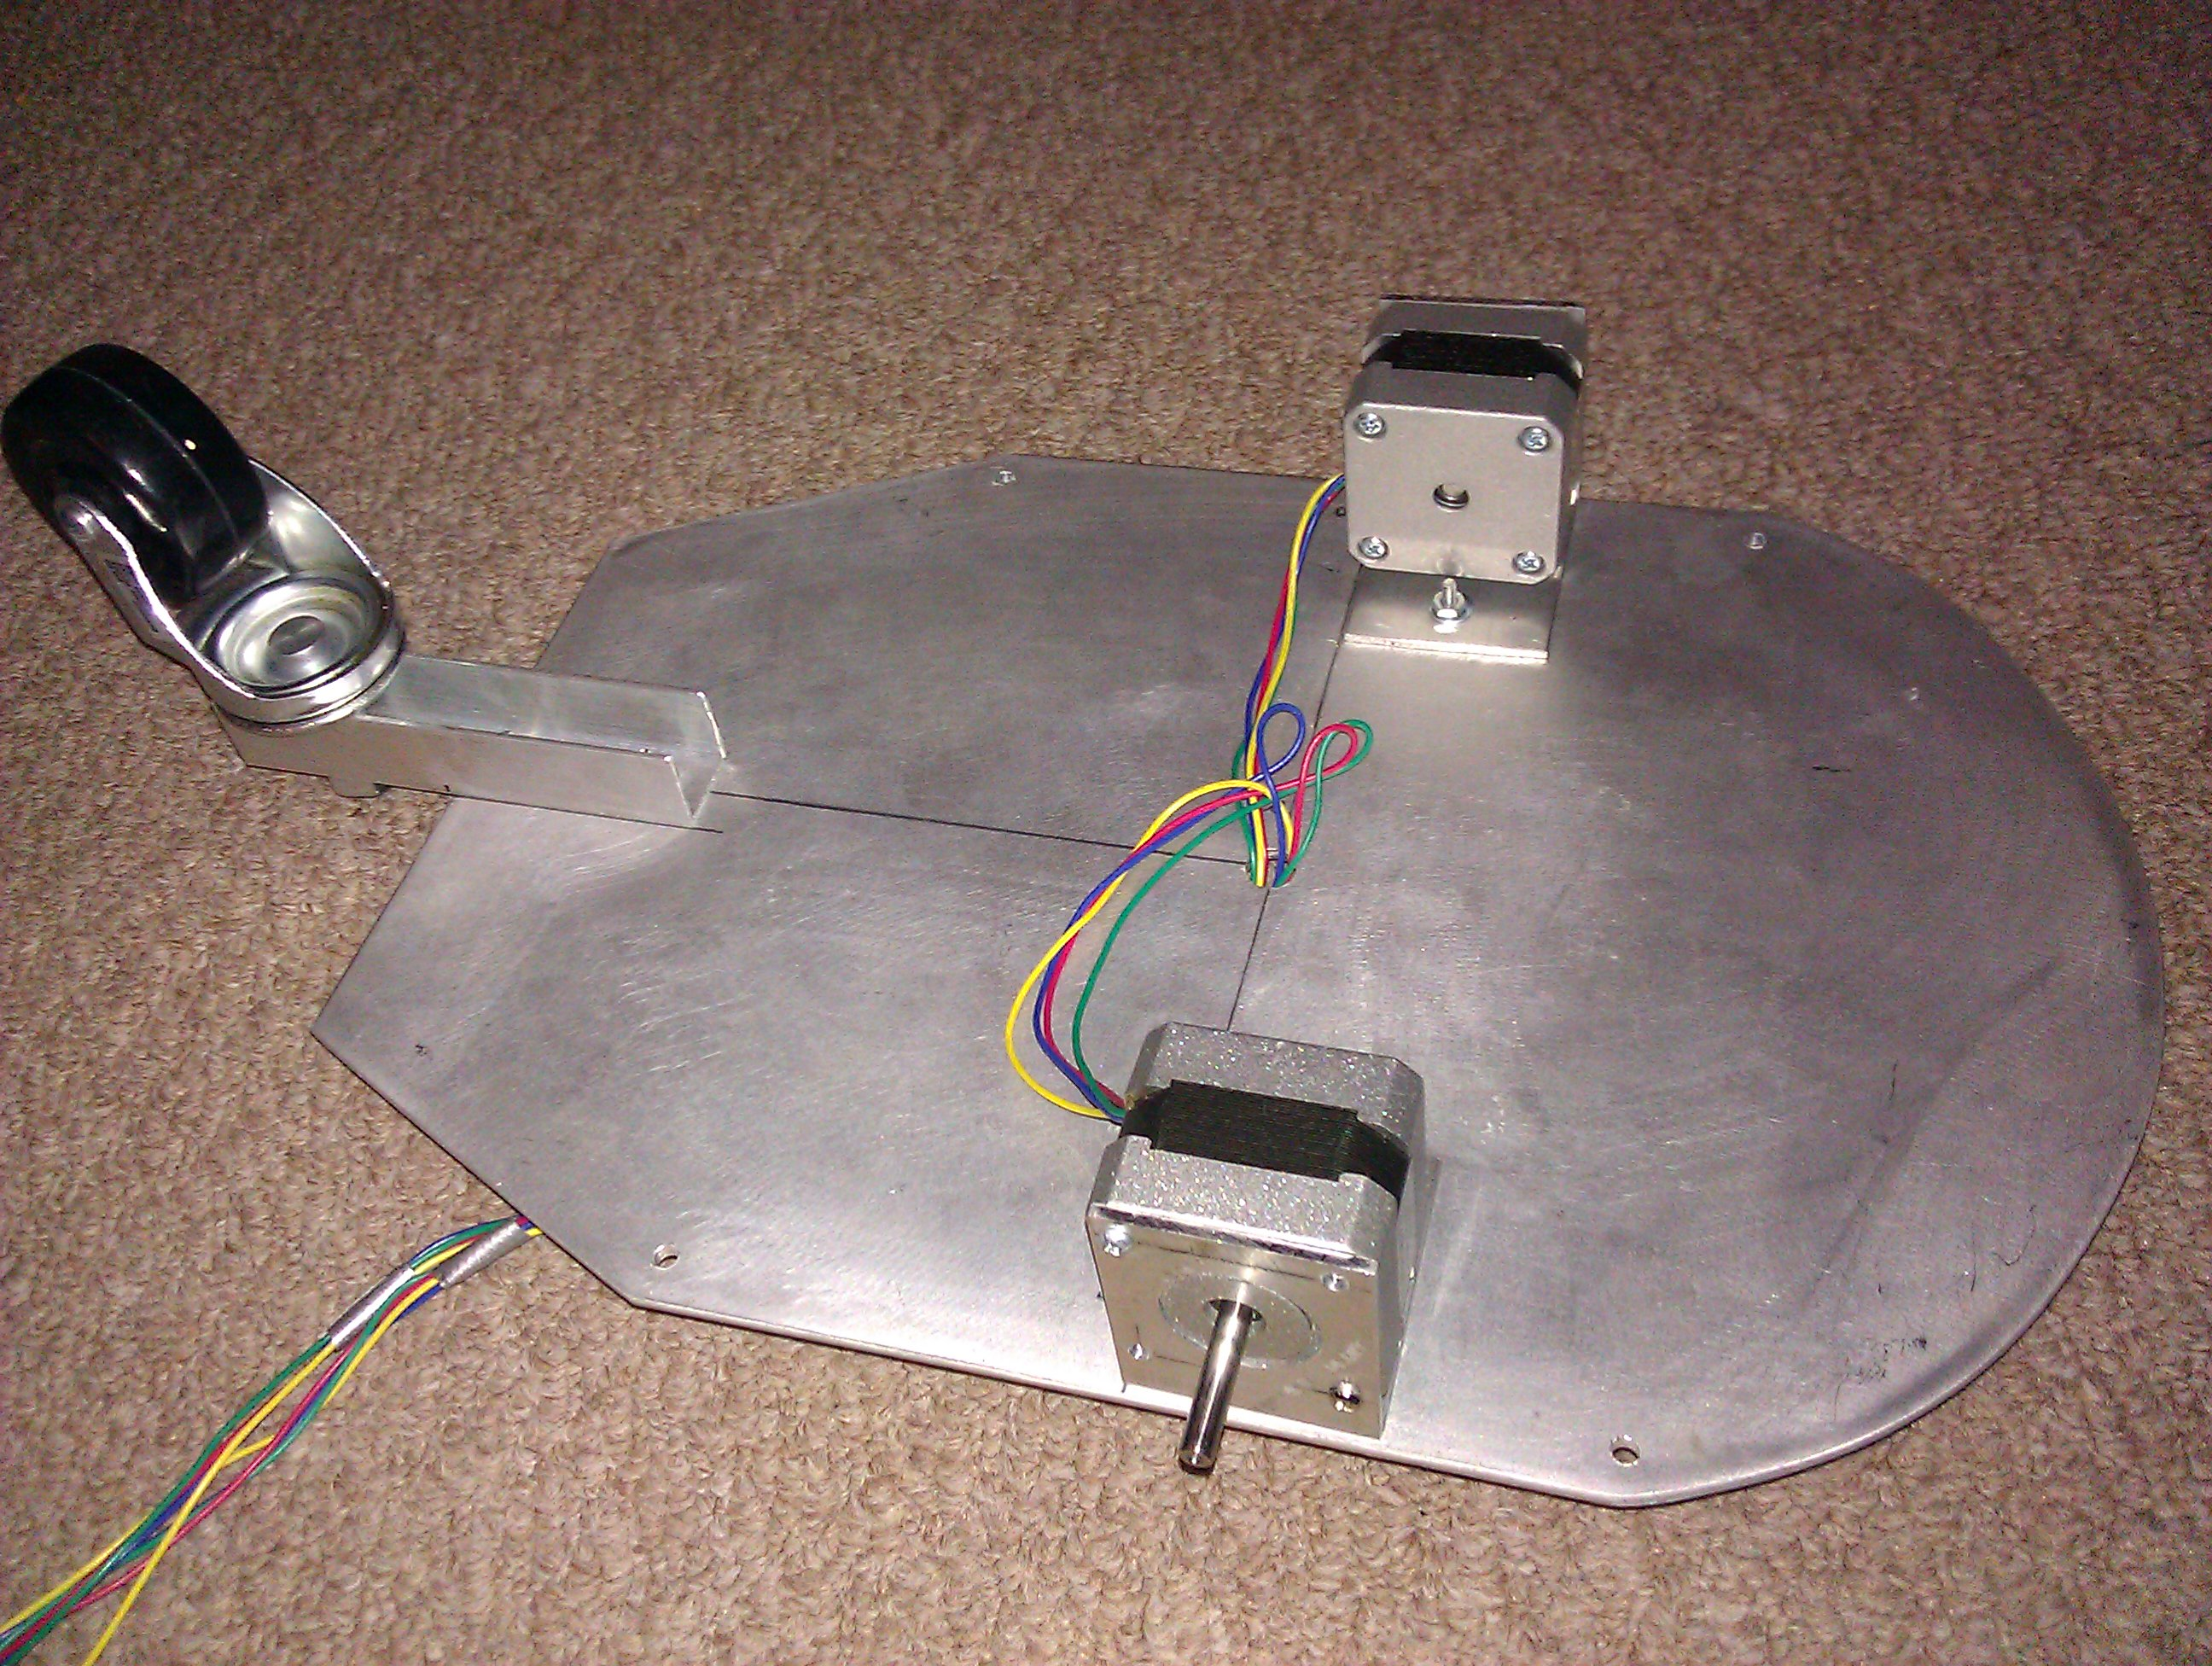
\includegraphics[width=5.0in] {figures/aluminium-chassis.jpg}
        \caption{Aluminium chassis}
        \label{Aluminium chassis}
\end{figure}

Using the 3d printer I made some mounting pieces to put electronic components onto the emtal chassis.  First something small and easy.  These are a sharpe infra red sensor mount and an ultrasonic sensor mount, the models for which I downloaded off of thingiverse.
%add thingiverse reference
\begin{figure}[h]
\centering
        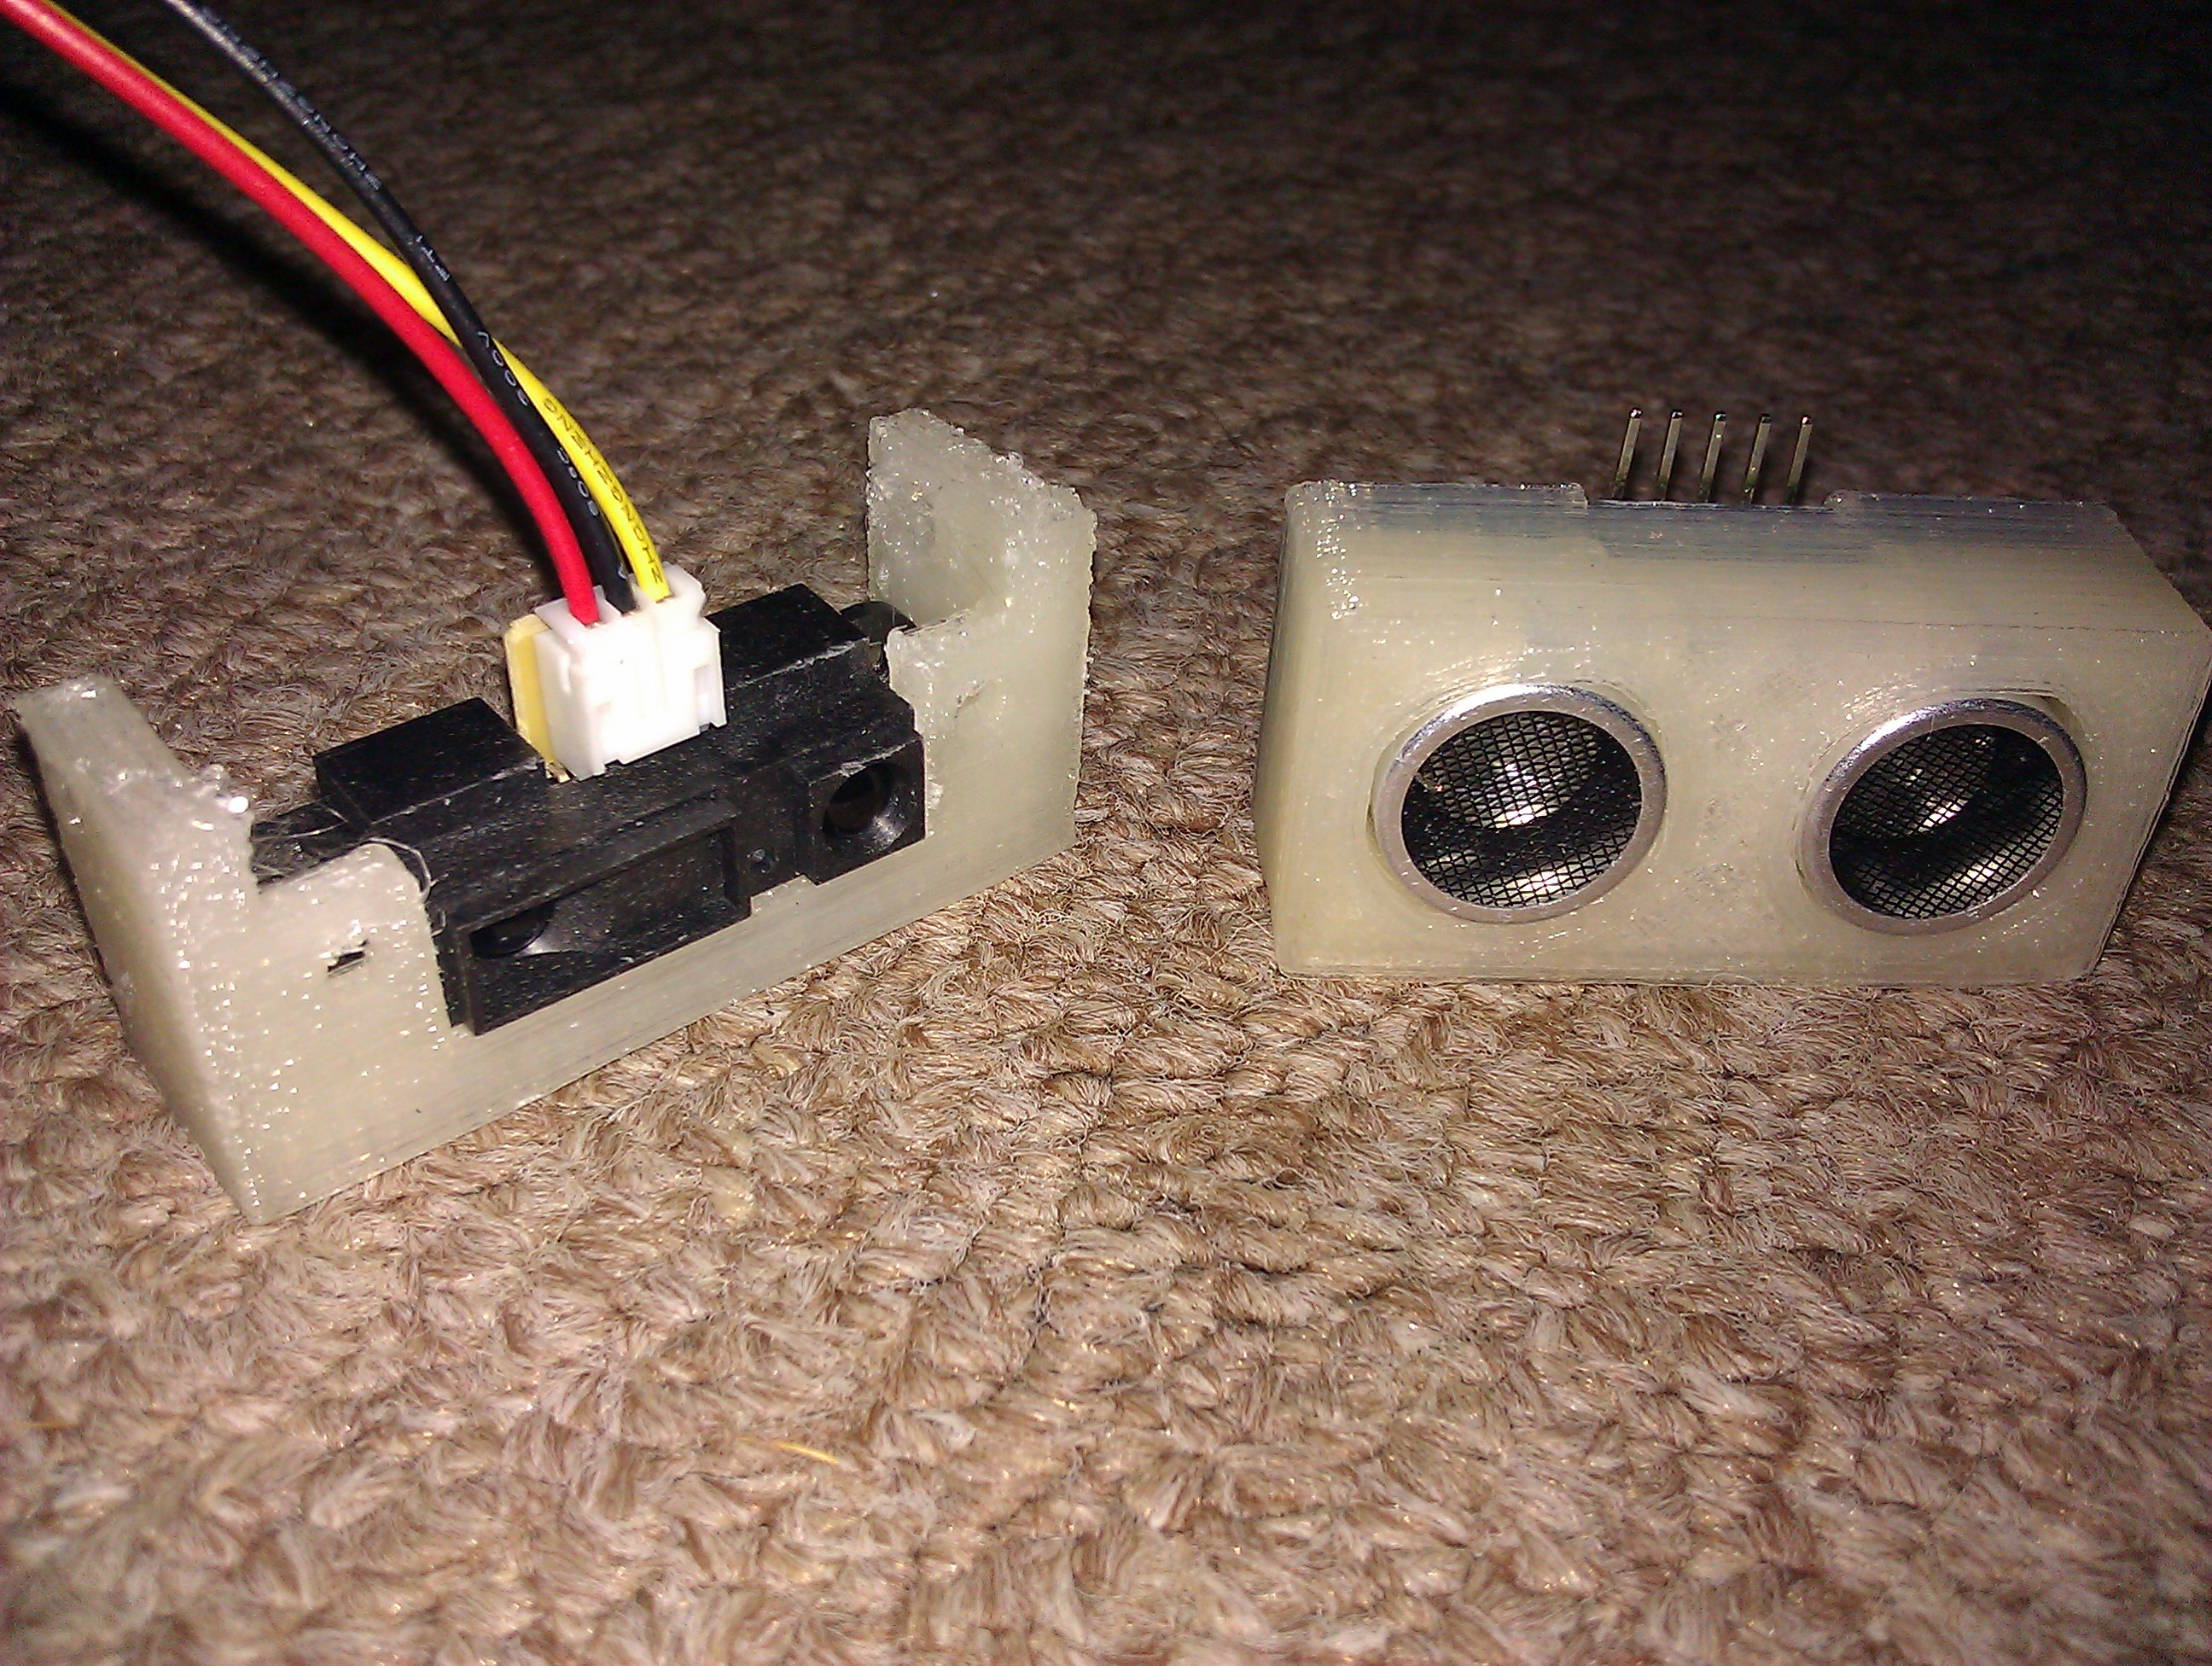
\includegraphics[width=3.0in] {figures/printed-sensor-mounts.jpg}
        \caption{Printed sensor mounts}
        \label{Printed sensor mounts}
\end{figure}




\subsection{Utility}
I put a small amount of time into building a portable device to interact with the main robot with main the purpose of reading live debug output.  This device was thought of because following aroudn the prototype with a laptop plugged into it became very anoying and quite awkward because if the robot made a tight turn it could get tangled up in the cable.

%==============================================================================
\section{Planning}
%==============================================================================


\nocite{*} % include everything from the bibliography, irrespective of whether it has been referenced.

% the following line is included so that the bibliography is also shown in the table of contents. There is the possibility that this is added to the previous page for the bibliography. To address this, a newline is added so that it appears on the first page for the bibliography.
\newpage
\addcontentsline{toc}{section}{Annotated Bibliography}

%
% example of including an annotated bibliography. The current style is an author date one. If you want to change, comment out the line and uncomment the subsequent line. You should also modify the packages included at the top (see the notes earlier in the file) and then trash your aux files and re-run.
%\bibliographystyle{authordate2annot}
\bibliographystyle{IEEEannot}
\renewcommand{\refname}{Annotated Bibliography}  % if you put text into the final {} on this line, you will get an extra title, e.g. References. This isn't necessary for the outline project specification.
\bibliography{mmp} % References file


\end{document}
